% 2009 年安徽卷文科第 17 题：按原卷印出的 24 个亩产数据填写的茎叶图（解答用）。
% 来源 PDF：普通高考/2009/2009安徽文.pdf，SHA256 83b982d22fd84a0158f909bce3d1f62e1fa228868e7915ded21e7a5ed9774897
% 原页：第 1 页（A3 三栏）第 3 栏下部，印刷页 497；题目数据见第 3 栏上部。
% 重绘依据：茎为十位与百位（35–45），叶为个位；A、B 两列按数据升序排列，逐项照录。
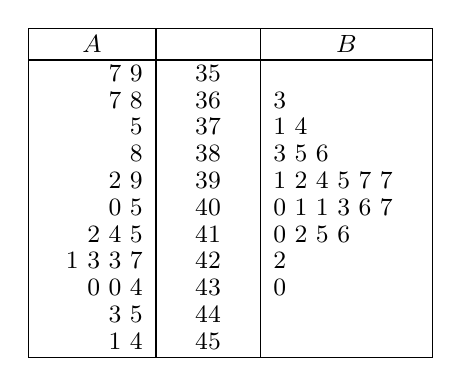
\begin{tikzpicture}[scale=0.95, semithick, every node/.style={inner sep=2.2pt, font=\small}]
  \draw (0,0) rectangle (5.4,-4.4);
  \draw (1.7,0) -- (1.7,-4.4);
  \draw (3.1,0) -- (3.1,-4.4);
  \draw (0,-0.42) -- (5.4,-0.42);
  \node at (0.85,-0.21) {$A$};
  \node at (4.25,-0.21) {$B$};
  \foreach \i/\s/\l/\r in {%
    0/35/{7\ 9}/{},%
    1/36/{7\ 8}/{3},%
    2/37/{5}/{1\ 4},%
    3/38/{8}/{3\ 5\ 6},%
    4/39/{2\ 9}/{1\ 2\ 4\ 5\ 7\ 7},%
    5/40/{0\ 5}/{0\ 1\ 1\ 3\ 6\ 7},%
    6/41/{2\ 4\ 5}/{0\ 2\ 5\ 6},%
    7/42/{1\ 3\ 3\ 7}/{2},%
    8/43/{0\ 0\ 4}/{0},%
    9/44/{3\ 5}/{},%
    10/45/{1\ 4}/{}} {
    \node[anchor=center] at (2.4,{-0.42-(\i+0.5)*0.358}) {$\s$};
    \node[anchor=east] at (1.62,{-0.42-(\i+0.5)*0.358}) {$\l$};
    \node[anchor=west] at (3.18,{-0.42-(\i+0.5)*0.358}) {$\r$};
  }
\end{tikzpicture}
